\documentclass{article}

\usepackage[utf8]{inputenc}

% Packages
\usepackage{amsmath,amssymb}
\usepackage{bm}% boldmath
\usepackage{listings} % Code block (source code) \begin{lstlisting} 
\usepackage{natbib}
\usepackage{graphicx}
\usepackage{lmodern}
\usepackage[usenames,dvipsnames,svgnames,table]{xcolor}
\usepackage[textwidth=16cm,textheight=23cm]{geometry}

%\usepackage{inconsolata} % New monospace font

% URL
\usepackage{url}
\usepackage[colorlinks=true, a4paper=true, pdfstartview=FitV, linkcolor=blue, citecolor=blue, urlcolor=blue]{hyperref}

% Figures
\usepackage[font=small, labelfont=bf]{caption}
\usepackage{subfig} % Subfigures. Uses \subfloat[captions text]{figure}

% Tables
\usepackage{booktabs}   % Allows the use of \toprule, \midrule and \bottomrule in tables for horizontal lines
\newcommand{\ra}[1]{\renewcommand{\arraystretch}{#1}} % spaces in tables

% Itemize
\usepackage{enumitem}

% Commands
%\newcommand{\code}[1]{\texttt{#1}} % \code{inline code}
\newcommand{\code}[1]{{\small\ttfamily #1}} % \code{inline code}
\newcommand{\expval}[1]{\langle #1 \rangle} %
\renewcommand{\theequation}{\arabic{section}.\arabic{equation}} % Book format equation
\renewcommand{\thefigure}{\arabic{section}.\arabic{figure}} % Book format figure
\renewcommand{\vec}[1]{{\bf #1}} % Lars likes this better than arrow

% Set page attribution
\setlength{\parindent}{0pt}


% PSTRICKS
\usepackage{pstricks,pst-node,pst-tree} % includes graph additions
\usepackage{pst-pdf} % Compiles the pictures
\usepackage{pst-node}
\usepackage{pst-plot}
\usepackage{pst-3dplot}
%\usepackage{pstricks-add,babel}




\lstset{
language=Python,                        % Code langugage
commentstyle=\color{gray},              % Comments font
basicstyle=\small\ttfamily,             % Code font, Examples: \footnotesize, \ttfamily
keywordstyle=\bfseries\color{blue},
stringstyle=\color{orange},
numbers=left,                           % Line nums position
numberstyle=\tiny,                      % Line-numbers fonts
stepnumber=1,                           % Step between two line-numbers
numbersep=5pt,                          % How far are line-numbers from code
frame=none,                             % A frame around the code
tabsize=4,                              % Default tab size
captionpos=b,                           % Caption-position = bottom
breaklines=true,                        % Automatic line breaking?
breakatwhitespace=false,                % Automatic breaks only at whitespace?
showspaces=false,                       % Dont make spaces visible
showstringspaces=false,                 % Dont make spaces visible in strings
showtabs=false,                         % Dont make tabls visible
belowskip=8pt,
morekeywords={range, xrange},
% backgroundcolor=\color{yellow}
% emph={[2]root,base}
% morekeywords={one,two,three,four,five,six,seven,eight,
}


%commentstyle=\color{gray},              % Comments font
%basicstyle=\small,                      % Code font, Examples: \footnotesize, \ttfamily



%basicstyle=\footnotesize\ttfamily,
%keywordstyle=\bfseries\color{green!40!black},
%commentstyle=\itshape\color{purple!40!black},
%identifierstyle=\color{blue},
%stringstyle=\color{orange},






\usepackage{multicol} % \begin{columns}

% ***************************************************
% HEADER INFORMATION

\title{Matplotlib Introduction}
\author{Molecular Statistics}
\date{2014}

% ***************************************************

\begin{document}

% ***************************************************
% BEGIN DOCUMENT
% ***************************************************

\maketitle

\section{Introduction}

{\bf Matplotlib} (MPL) is a module for Python used for plotting.
It is very useful for visualizing all kinds of data types and is extremely customizable.
For plot examples see 
\href{http://matplotlib.org/gallery.html}{matplotlib.org/gallery.html} and
\href{http://webloria.loria.fr/~rougier/teaching/matplotlib/}{webloria.loria.fr/\~{}rougier/teaching/matplotlib}. \\

This short introduction will go through small plots with code examples. For advanced examples (like 3D plots), see the examples above or use "Google".\\

To utilize the power of matplotlib in a simple way we use a wrapper function called {\bf pyplot} (PLT), which basically means that we can use matplotlib without any crazy coding (involving classes and instances etc).
This is simply done by importing the pyplot module in the head of your \code{.py} file.

\begin{lstlisting}
import numpy as np
import matplotlib.pyplot as plt
\end{lstlisting}

After creating a plot, there are several ways to show the results. You can either open a window to show the plot or save the plot as an image or another format.

\begin{lstlisting}
plt.show()                  # Show the plot in a new window
plt.savefig('my_plot.png')  # Save the plot in a file
\end{lstlisting}

% Full list:
% emf, eps, jpeg, jpg, pdf, png, ps, raw, rgba, svg, svgz, tif, tiff

The \code{savefig()} function can save to
\code{.png},
\code{.eps},
\code{.svg},
as well as
\code{.pdf} formats, which are very useful for use in {\LaTeX}.\\

When working with multiple plots in the same script, remember to clear the plot data after each figure is shown or saved, or you will see a mess of data in your plots. This is done using the \code{clf()} function from PLT.

\begin{lstlisting}
plt.clf()
\end{lstlisting}

If you want to make you graphs look good with different colors, fonts and spacings, then I would recommend you to look at 
\href{http://github.com/charnley/matplotlib-header}{github.com/charnley/matplotlib-header}
and
\href{http://matplotlib.org/users/customizing.html}{matplotlib.org/users/customizing.html}.\\

Happy Pyplot'ing!\\



\newpage
\section{Examples}

\subsection{XY}

A simple example is to plot $x$ and $y$ coordinates based on two simple python lists.
For $y(x) = x^2$.

\begin{multicols}{2}

    \lstinputlisting{py/xy_figure.py}

\columnbreak

    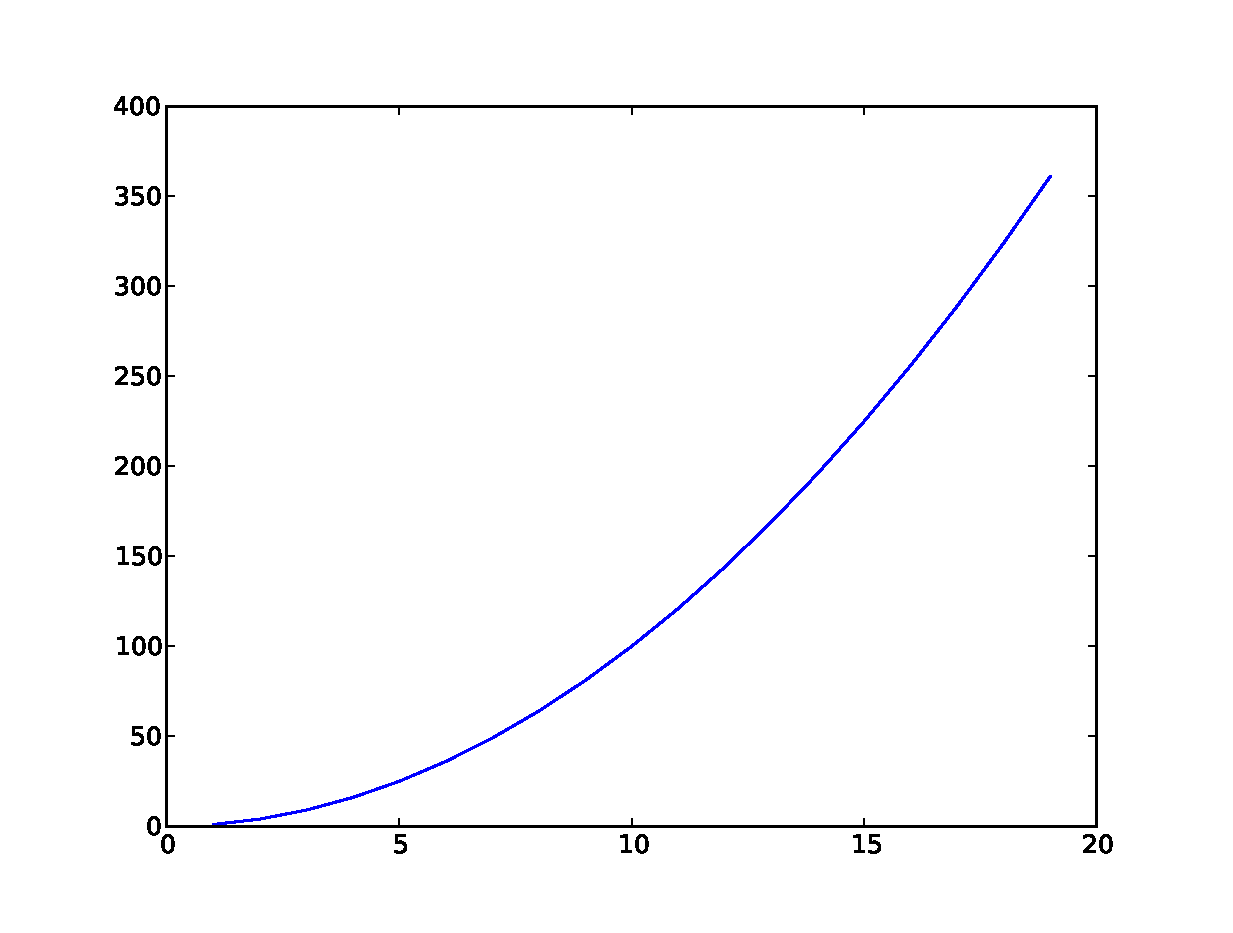
\includegraphics[width=1.0\linewidth]{py/figure_xy.eps}

\end{multicols}


\newpage
\subsection{Titles and labels}

However a graph is worth nothing without title and axis-labels,
which can be included by the following syntax.
It is also possible to include latex code in the strings.

\begin{multicols}{2}

    \lstinputlisting{py/xy_figure_title.py}

\columnbreak

    \centering

    figure\_title.eps

    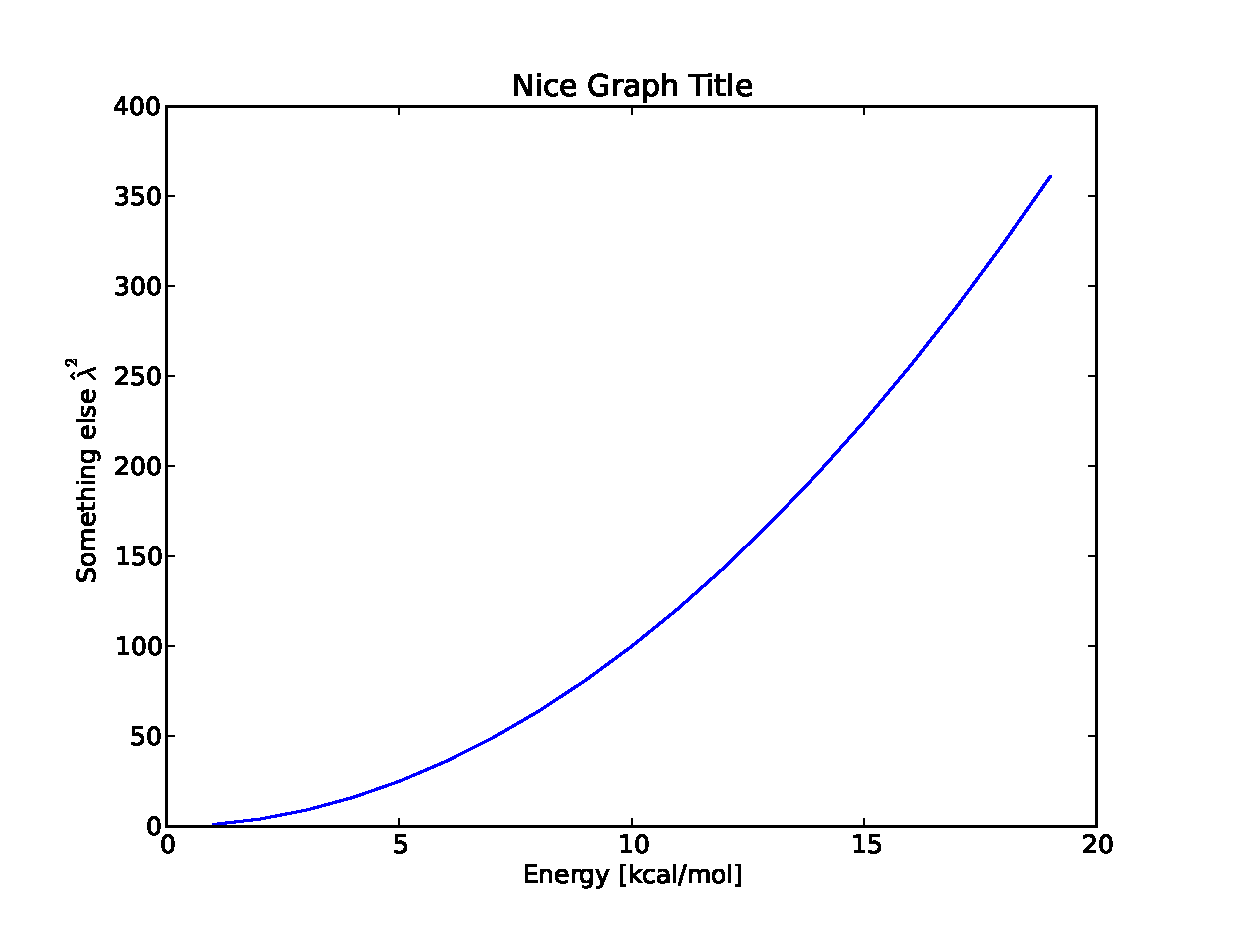
\includegraphics[width=1.0\linewidth]{py/figure_title.eps}

    figure\_title\_text.eps

    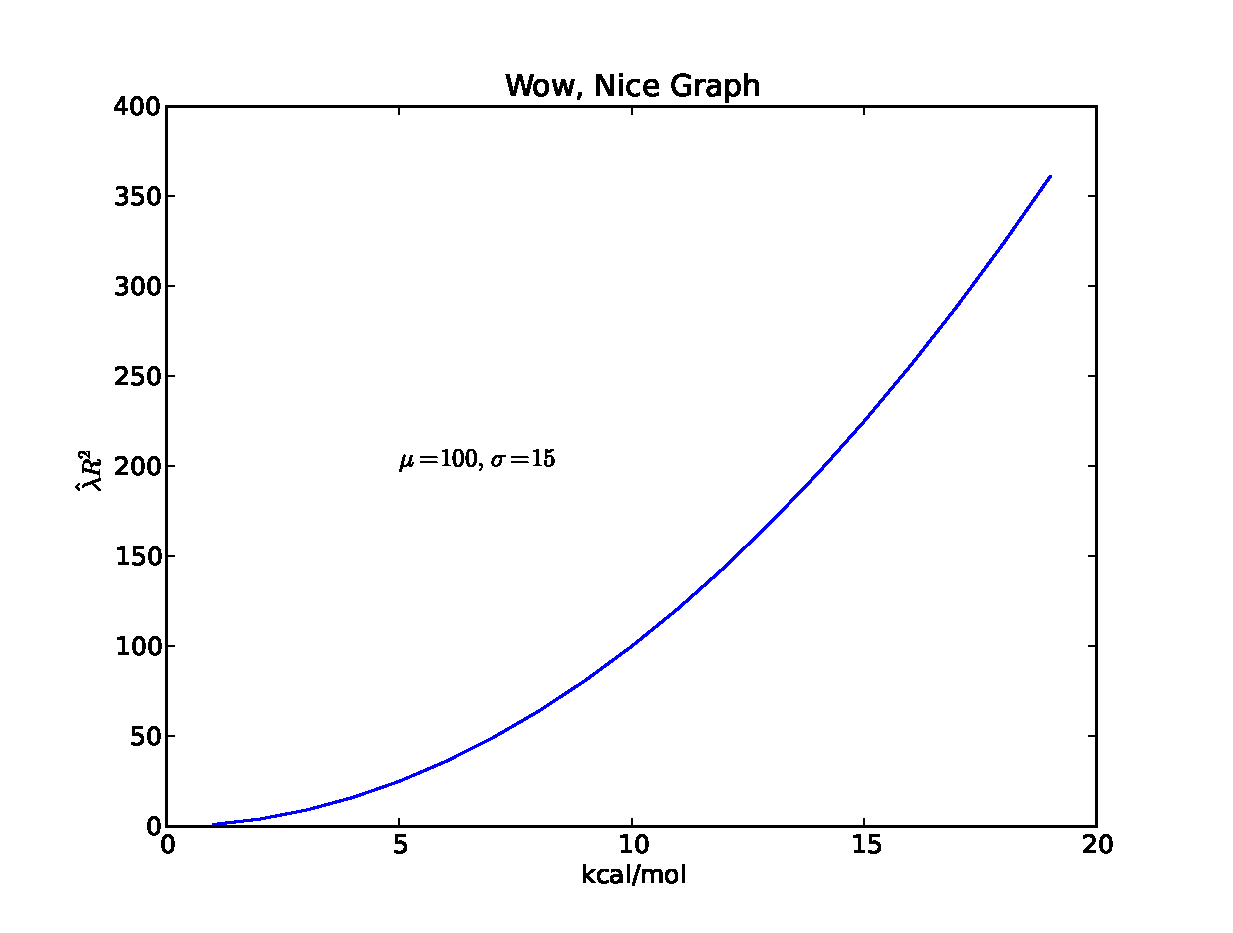
\includegraphics[width=1.0\linewidth]{py/figure_title_text.eps}

\end{multicols}


\newpage
\subsection{Multiple lines}

Usually you will need to plot multiple datasets in the same figure which is done
by adding more \code{plot()} functions.
For customization you can add labels and choose color and line-type for the specific data sets.
See appendix A for a full list of colors and line styles.
If you do not choose a color, a color will be chosen by default.\\

Note that the location of the legend box can be set by changing the string location.

\begin{multicols}{2}

    \lstinputlisting{py/xy_figure_labels.py}

\columnbreak

    \centering

    figure\_sincos2.eps

    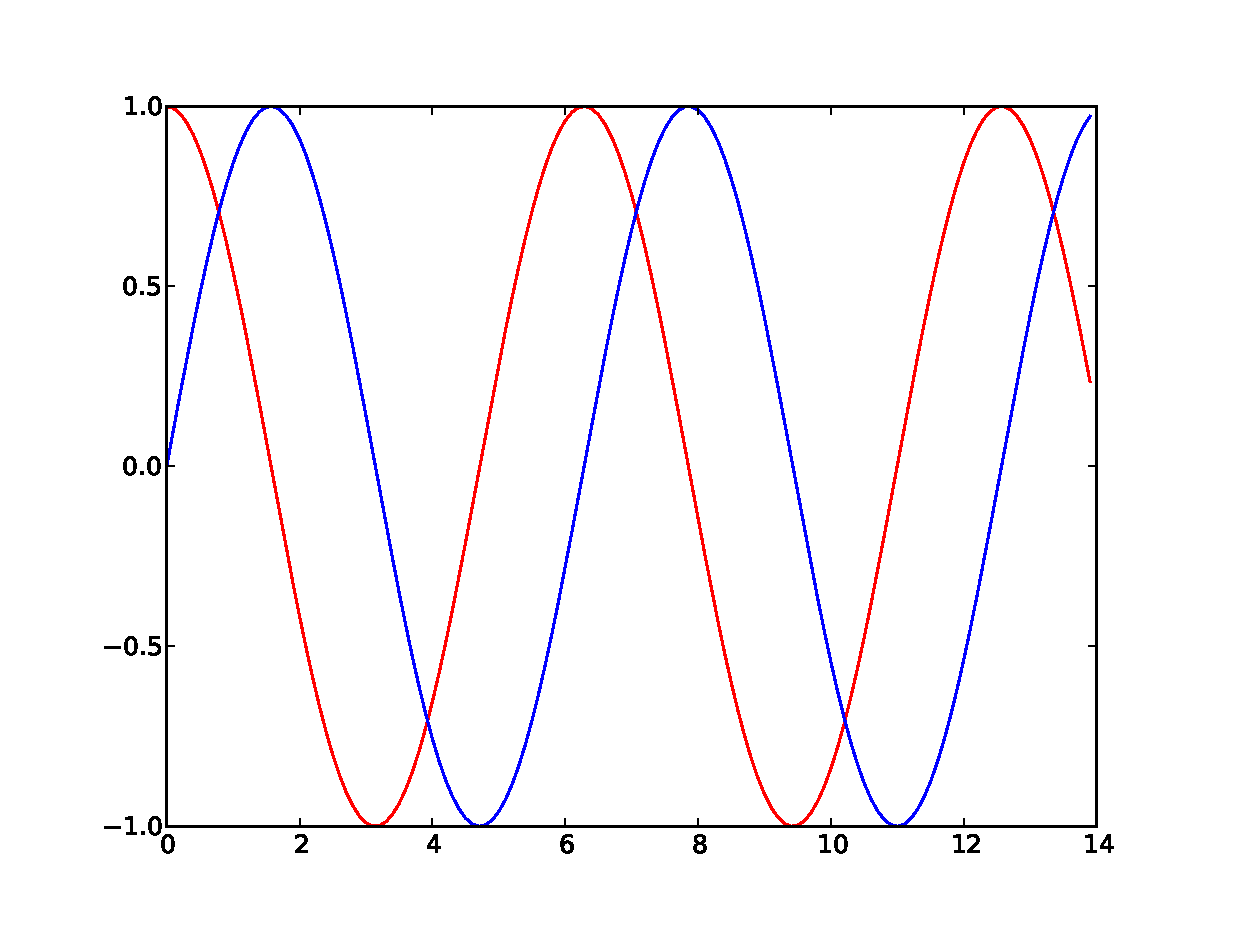
\includegraphics[width=1.0\linewidth]{py/figure_sincos1.eps}

    figure\_sincos2.eps

    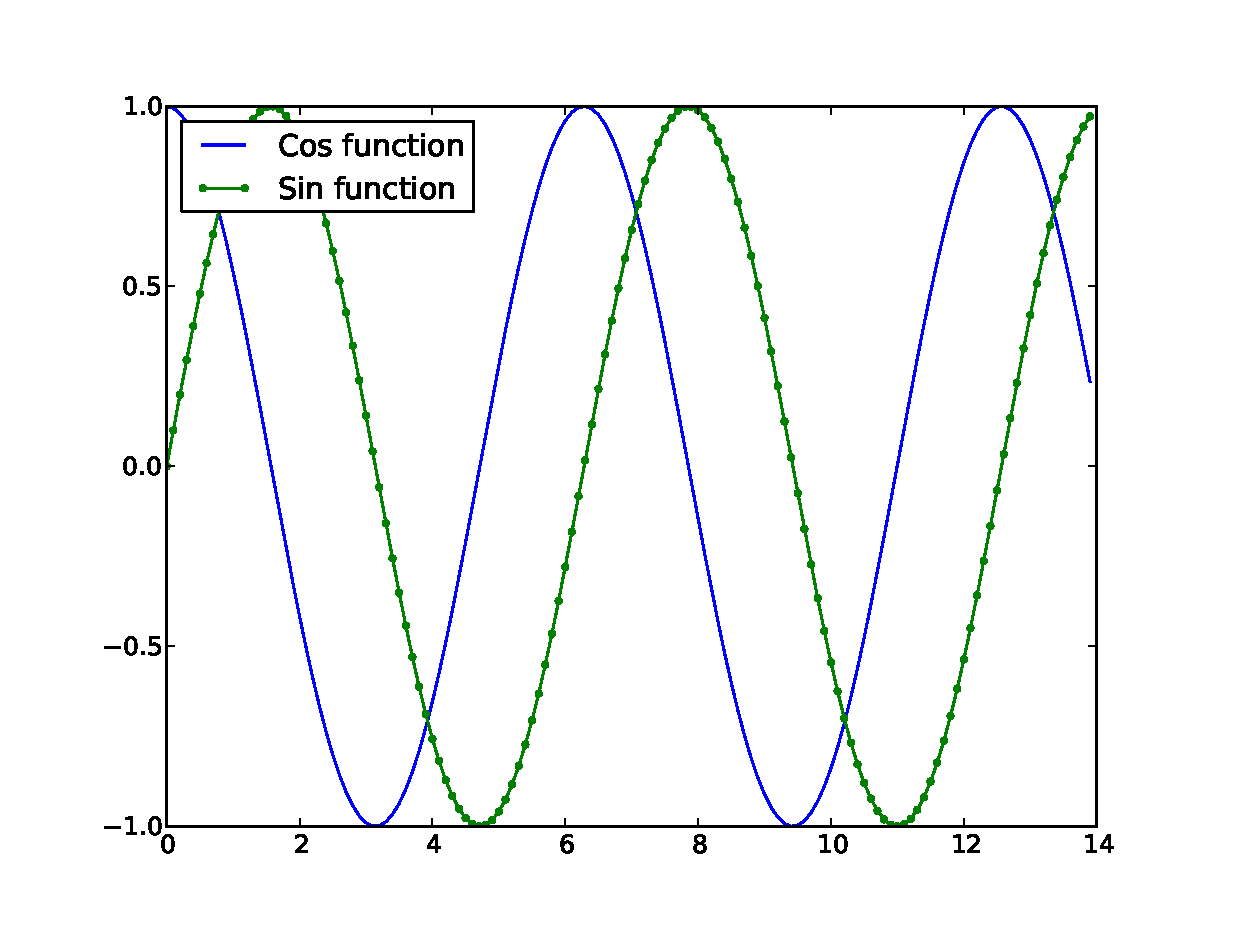
\includegraphics[width=1.0\linewidth]{py/figure_sincos2.eps}

\end{multicols}






%%%%%%%%%%%%%%%%%


% TODO EXAMPLES
% xlim(X.min()*1.1, X.max()*1.1)
%ylim(C.min()*1.1, C.max()*1.1)


% import matplotlib matplotlib.use("Agg")



\appendix
\newpage

\section{Plot styling}

\begin{multicols}{2}

    \subsection{Colors}

    \begin{tabular}{ l l }
    b & blue \\
    g & green \\
    r & red \\
    c & cyan \\
    m & magenta \\
    y & yellow \\
    k & black \\
    w & white \\
    \end{tabular}

\columnbreak

    \subsection{Line styles}

    \begin{tabular}{ l l }
        0 & tickleft\\
        1 & tickright\\
        2 & tickup\\
        3 & tickdown\\
        4 & caretleft\\
        D & diamond\\
        6 & caretup\\
        7 & caretdown\\
        s & square\\
        | & vline\\
        x & x\\
        5 & caretright\\
        \_ & hline\\
        \^{} & triangle up\\
        d & thin diamond\\
        h & hexagon1\\
        + & plus\\
        * & star\\
        , & pixel\\
        o & circle\\
        . & point\\
        '1' & tri down\\
        p & pentagon\\
        '3' & tri left\\
        '2' & tri up\\
        '4' & tri right\\
        H & hexagon2\\
        v & triangle down\\
        '8' & octagon\\
        \textless & triangle left\\
        \textgreater & triangle right
    \end{tabular}

\end{multicols}



% ***************************************************
% END DOCUMENT
% ***************************************************

\end{document}

